\section{Implementation}\label{sec:impl}
To alleviate the shortcoming of the old playback and trace buffer design it is fundamentally redesigned.
There are four operations that need to be performed by the playback and trace buffer:
\begin{enumerate}
  \item Playback instructions sent by the host have to be written to the \DDR{} memory.
  \item The playback instructions received previously from the host have to transferred to the \pbexec{}.
  \item The trace data generated by the \pbexec{} has to be written to the \DDR{} memory.
  \item Trace data has to read from the \DDR{} memory and sent back to the host.
\end{enumerate}
These operations can be grouped into two categories: First host-side operations, which includes the first and the last of the four listed operations. The operations in this category allow the host to read and write the \DDR{} memory.
The second category is \FPGA{}-side operations, which includes the second and third operation listed. The operations in this category are responsible for reading and writing to the \DDR{} memory to generate the playback instructions stream for the \pbexec{} and to store the trace data generated by the \pbexec{}.
The first category of operations will be implemented using the \FAXI{} unit to allow memory mapped read and write access to the whole \DDR{} memory by the host.
To implement the second category of operations a scatter gather \DMA{} engine to on the one hand assembly the playback stream for the \pbexec{} from data that was written by the host to the \DDR{} memory and on the other hand to store the trace data transmitted by the \pbexec{} to the \DDR{} memory will be used

\autoref{fig:detail_new} shows a schematic overview of the replacement block developed in this thesis.

\begin{figure}[htbp]
\centerline{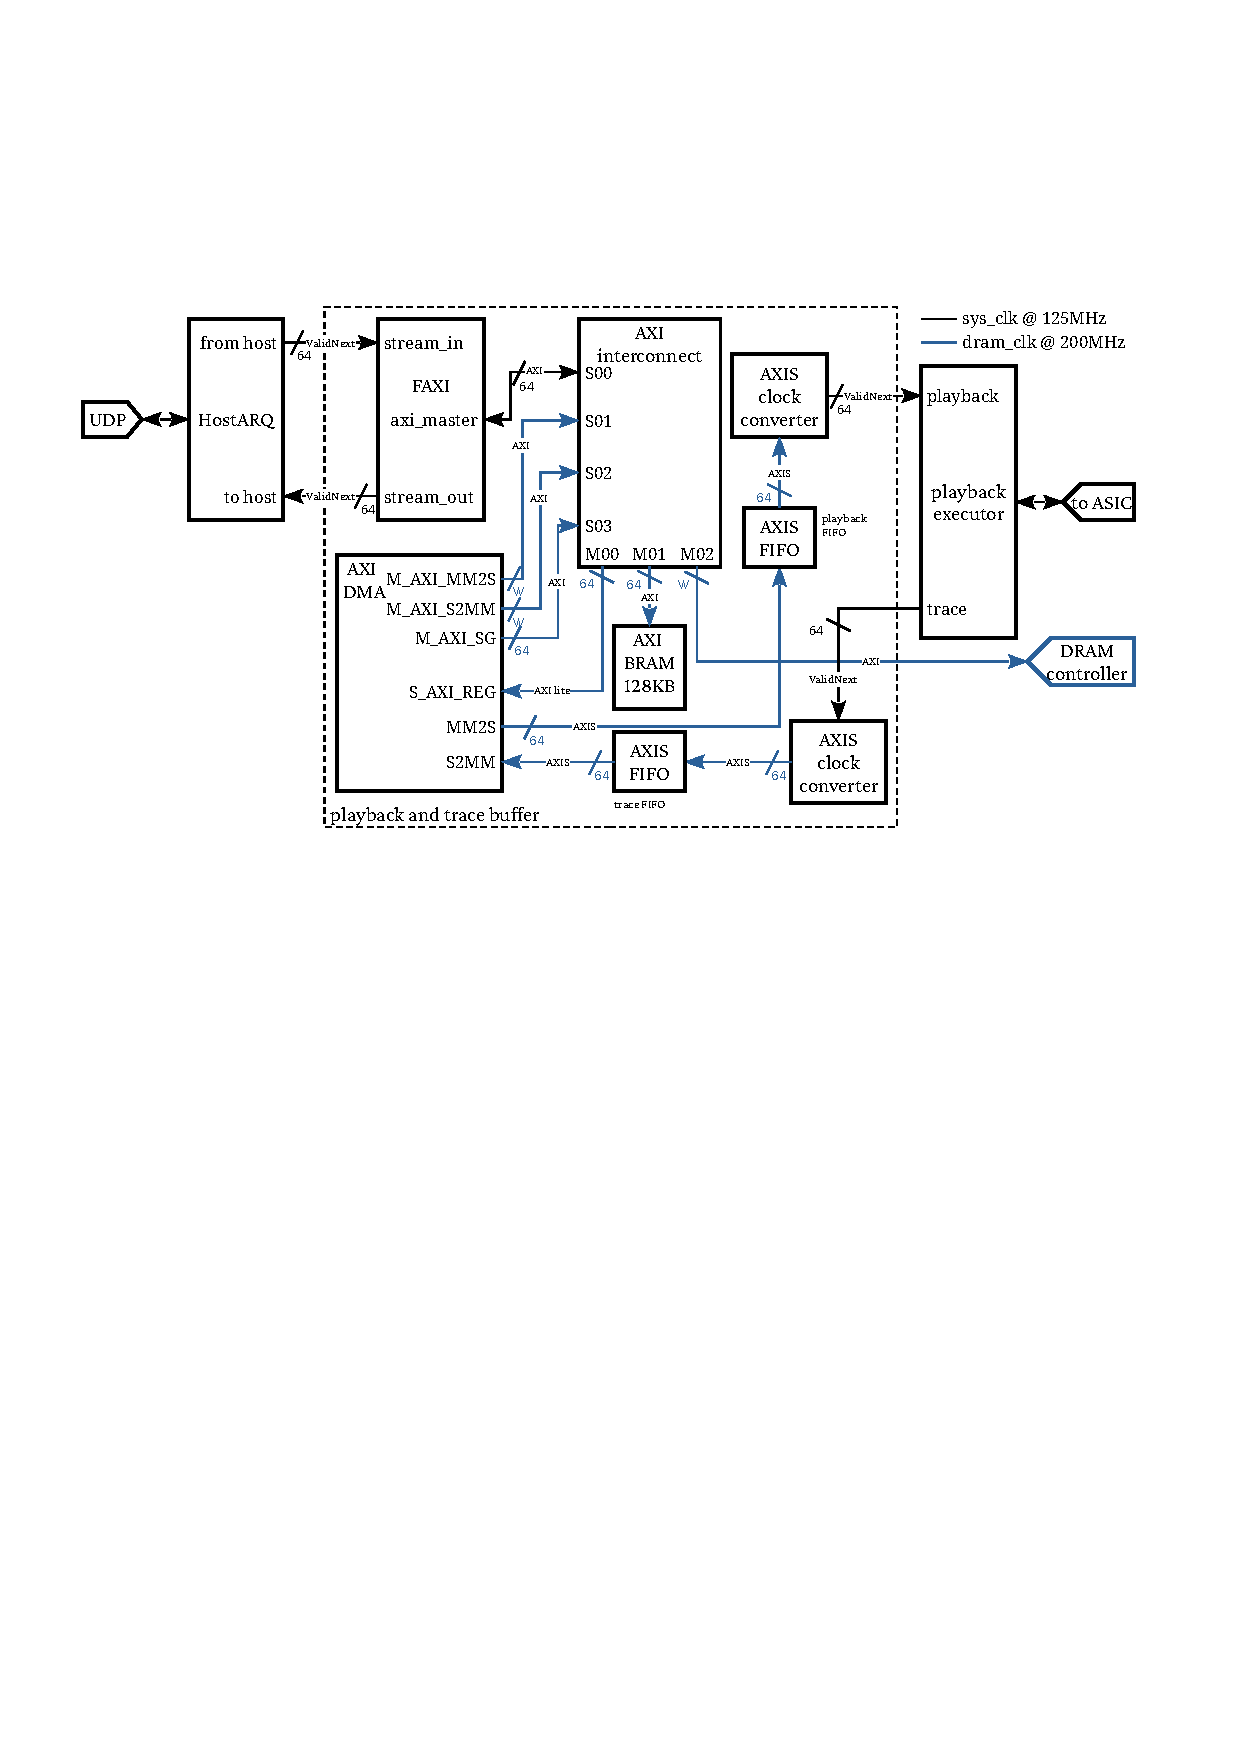
\includegraphics{diagrams/cropped/detail_new}}
\caption{Schematic overview of the new playback and trace buffer. Instead of implementing two \FIFO{}s it allows direct read and write access to the \DDR{} memory by the host. A scatter gather \DMA{} engine is used to read from the \DDR{} memory and transmit the read data as the playback stream to the \pbexec{} as well as writing the trace data from the \pbexec{} to the \DDR{} memory.}\label{fig:detail_new}
\end{figure}

\subsection{FAXI}
To allow the host to read and write to the \DDR{} memory the \FAXI{} unit is used. This unit was developed by the Electronic Vision(s) group for a different \FPGA{} design. It implements a bridge between the \HostARQ{} \FPGA{} interface of two \PhyWordSize{} wide streams and an \AXI{} Subordinate with data width of \PhyWordSize{} and an address size of \PhyWordSize{}.
Read and write requests are encoded in the \HostARQ{} stream using a \PhyWordSize{} header controlling the kind of operation (read or write) and the \burstsize{}. This header is followed by a \PhyWordSize{} address and for a write requests by the specified number of \PhyWordSize{} words.
Read data and write response is sent back to the host following a similar scheme of a \PhyWordSize{} header followed by the read data words.
Finally, \FAXI{} supports a \globalfence{} operation, that blocks the processing of the further data until every outstanding read or write transaction is completed.

The subset of \AXI{} that is supported by it is summarized in \autoref{tbl:faxi_axi_features}.

\begin{table}
  \begin{center}
\begin{tabular}{ll}
  \toprule
  feature & status  \\
  \midrule
  data width & $\SI{64}{\bit}$ \\
  address width & $\SI{64}{\bit}$ \\
  transaction ID & not supported \\
  AxLOCK & not supported \\
  AxCACHE & not supported \\
  AxPROT & not supported \\
  AxQOS & not supported \\
  AxREGION & not supported \\
  user signals & not supported \\
  narrow transfers & not supported \\
  write strobe & partially, see description \\
  \bottomrule
\end{tabular}

  \end{center}
\caption{Summary of the \AXI{} features supported by \FAXI{}. \AXI{} usually allows a different write strobe for each data word of a write transaction. \FAXI{} only allows a fixed write strobe for a complete write transaction.}\label{tbl:faxi_axi_features}
\end{table}

\HostARQ{} is configured to use a maximum packet size of $\num{180}$ words with $\PhyWordSize{}$ per words.
Each packet has an overhead of $\SI{78}{\byte}$ from the \Gigabitethernet{}, IPv4, \UDP{} and \HostARQ{}.
The maximum burst length of an \AXI{} write is $\num{256}$ words and to encode a write-burst \FAXI{} has an overhead of two $\PhyWordSize{}$ words (the header and the address). From the maximum data rate $\SI{1}{\giga\bit\per\second}$ of \Gigabitethernet{} one obtains for the maximum write bandwidth possible
\[
B_{\text{\FAXI{},w}} = \num{180} · \PhyWordSize{} \frac{\SI{1}{\giga\bit\per\second}}{\SI{78}{\byte} + 180 · \PhyWordSize{}} · \frac{256 \PhyWordSize{}}{(256 + 2) \PhyWordSize{}} \approx \SI{112.21}{\mebi\byte\per\second}
\]
For a read the overhead due to the \FAXI{} encoding is only one \PhyWordSize{} word and one obtains
\[
B_{\text{\FAXI{},w}} = \num{180} · \PhyWordSize{} \frac{\SI{1}{\giga\bit\per\second}}{\SI{78}{\byte} + 180 · \PhyWordSize{}} · \frac{256 \PhyWordSize{}}{(256 + 1) \PhyWordSize{}} \approx \SI{112.64}{\mebi\byte\per\second}
\]


\subsection{AXIDMA}\label{sec:AXIDMA}
The \AXIDMA{} IP core by \Xilinx{}\autocite{ref:axidma} provides a \DMA{} engine. This is split into two separate channels, the \MMToS{} channel and the \SToMM{} channel.
The \MMToS{} channel is used to read data from an \AXI{} Subordinate and transmit the data using an \AXIStream{}. It is used to read the data written to the \DDR{} memory by the host using \FAXI{} and transmit it to the \pbexec{}. The \SToMM{} channel performs the opposite operation and writes data from an \AXIStream{} to an \AXI{} Subordinate. It is used to write the trace data received from the \pbexec{} to the \DDR{} memory.
Moreover, the \AXIDMA{} core has a separate set of \AXILite{} accessible registers that are used to control its operation.

The \AXIDMA{} \DMA{} engine can be used to perform scatter and gather operations. In the scatter gather mode the operation of these channels is controlled using a chain of \descriptor{}s.
Each \descriptor{} contains an address, a buffer length, the address of the next descriptor, as well as a status and a control field. For the \MMToS{} channel, the address specified in the descriptor is the address of the first byte that is read by the channel. The total number of consecutive bytes read from this address is specified by the buffer length. When every byte specified by the descriptor was read, the \AXIDMA{} sets the completed flag in the status field and, the next descriptor as specified by the next descriptor address is used to continue the operation. The control field contains a start and an end of frame flag. The latter is used to generate the \TLAST{} signal of the \AXIStream{} driven by the \MMToS{} channel. Operation of the \MMToS{} channel is started by writing the address of the first descriptor and the address of the last descriptor to the \curdesc{} and \taildesc{} registers of the \MMToS{} channel.

The \SToMM{} channel operates similarly. For each descriptor it writes up to the specified buffer length consecutive bytes from the \SToMM{} \AXIStream{} Receiver to the address specified in the descriptor.
Whenever the last word of a packet as specified by the \TLAST{} signal or the number of bytes specified by the buffer length was written, the completed flag as well as the number of transferred bytes is updated in the status field of the descriptor and the next descriptor is read from the specified address for the next descriptor.

The \AXIDMA{} core uses separate \AXI{} Managers for the \SToMM{} and the \MMToS{} channel as well as the scatter gather descriptors.

\subsection{New playback and trace buffer}
Using an \AXI{} interconnect like the \smartconnect{} allows operations from multiple \AXI{} Managers to be multiplexed to multiple \AXI{} Subordinates based on the address.
For the playback and trace buffer design it is used to allow access from \FAXI{} and both \AXIDMA{} channels to the \AXI{} interface of the \DDR{} controller.
\autoref{tbl:axi_memory_map} contains an overview of the memory map that was chosen. The interconnect is used to allow \FAXI{} to access the \DDR{} memory, the \AXIDMA{} registers and the scatter gather descriptor memory while also allowing both \AXIDMA{} channels to access the \DDR{} memory and \AXIDMA{} to access the scatter gather descriptor memory.

To store the scatter gather descriptors there are two options. One could use the main \DDR{} memory or a separate memory. Using a separate memory has several advantages. It ensures that interaction such as reading and writing the \descriptor{} cannot have any effect on the reads and writes to the \DDR{} memory performed by the \SToMM{} and \MMToS{} channels. Additionally, reads and writew to it have a lower latency than reads and writes to the \DDR{} memory.
Each \descriptor{} has a size of $\SI{64}{\byte}$, accordingly the $\SI{128}{\kibi\byte}$ memory used for the descriptors allows for up to $\num{2048}$ descriptors.

\begin{table}
\begin{center}
\begin{tabular}{llr}
\toprule
  \AXI{} Subordinate & address & size \\
  \midrule
  \DDR{} memory & $\texttt{0000\,0000}_{16}$ & \DDRSIZE{} \\
  scatter gather descriptor memory & $\texttt{A000\,0000}_{16}$ & $\SI{128}{\kibi\byte}$ \\
  \AXIDMA{} registers & $\texttt{B000\,0000}_{16}$ & $\SI{8}{\kibi\byte}$ \\
  \bottomrule
\end{tabular}
\end{center}
\caption{\AXI{} memory map.}\label{tbl:axi_memory_map}
\end{table}

As every address that is accessible according to the address map given in \autoref{tbl:axi_memory_map} can be represented with $\SI{32}{\bit}$ an address width of $\SI{32}{\bit}$ is used every \AXI{} bus.
The \AXIDMA{}, \XilinxMIG{}, \smartconnect{} and the \AXIBRAMController{} do not have an fixed \AXI{} data width but instead allow a variety of different configurations.
Their configuration was chosen to use the minimal width that satisfy the requirement of $\pbExecBandwidth{}$ bandwidth for the playback and the trace stream generated by the \MMToS{} and \SToMM{} channels. Minimizing the width directly reduces the required amount of \FPGA{} resources like \LUT{}s and \FF{}s and moreover reduces the number of routing resources. The \FPGA{} design is limited by these routing resources\autocite{ref:fpga_routing_limited}.
As described in \autoref{sec:AXI} the theoretical maximum data rate of an \AXI{} bus is determined by the clock frequency and the data width.

There are three choices for the clock
\begin{enumerate}
    \item The $\SI{125}{\mega\hertz}$ clock shared by the \HostARQ{} and the \pbexec{}.
    \item The same clock as the \XilinxMIG{} memory interface.
    \item A clock not shared with any of the ports
\end{enumerate}
The second option was selected with the \XilinxMIG{} operating in 2:1 mode resulting in a clock frequency of $\SI{200}{\mega\hertz}$. Using the 2:1 mode instead of the 4:1 mode with a clock frequency of $\SI{100}{\mega\hertz}$ halves the required data width as the clock frequency is doubled. For the same region using the $\SI{200}{\mega\hertz}$ was preferred over the $\SI{125}{\mega\hertz}$ clock of the \HostARQ{} and \pbexec{} interfaces.
% \todo{maybe something about how it actually manages to implement them at 200mhz and we therefore do not need to use a slow clock domain?}
Furthermore, using a clock that is shared with some ports of the module reduces the required clock domain crossing logic.

The \SToMM{} an \MMToS{} \AXIStream{}s are configured to use a data width of \PhyWordSize{}. At clock frequency of $\SI{200}{\mega\hertz}$ this results in a bandwidth of $\SI{12.8}{\giga\bit\per\second}$, satisfying the minimum requirement of \pbExecBandwidth{}. By choosing the same data width the \pbexec{} playback and trace streams no width conversion is necessary. For the bandwidth that can actually be achieved by the \AXIDMA{} only limited information is provided by \Xilinx{}. \Xilinx{} specifies that an \AXIDMA{} operating at a clock frequency of $\SI{100}{\mega\hertz}$ is able to achieve $\SI{99.76}{\percent}$ of the theoretical throughput on the \MMToS{} channel and $\SI{74.64}{\percent}$ of the theoretical throughput on the \SToMM{} channel when transferring $\SI{10000}{\byte}$\autocite{ref:axidma}. Assuming the relative throughput is independent of the clock frequency operation a $\SI{200}{\mega\hertz}$ should be able to achieve a bandwidth greater than the requirement of $\pbExecBandwidth{}$.

For the data width $W$ of the remaining \XilinxMIG{} \AXI{} Subordinate interface and the \SToMM{} and \MMToS{} \AXI{} Manager a choice of \PhyWordSize{} and $\SI{128}{\bit}$ is evaluated.

\Xilinx{} specifies that the bandwidth achievable by the \XilinxMIG{} will vary depending on the access pattern and other system parameters. It is of course limited by the maximum bandwidth that is achievable using the \DDR{} interface of the memory. An upper bound of this bandwidth $B_{\text{\DDR{}}}$ can be determined from the clock frequency the memory is operated at $f_{\text{\DDR{}}} = \SI{400}{\mega\hertz}$ and the number of data lanes $n_{\text{dq}} = \num{32}$
\[B_{\text{\DDR{}}} = 2 f_{\text{\DDR{}}} n_{\text{dq}} · \SI{1}{\bit} = \SI{25.6}{\giga\bit\per\second}\]
This upper bound is not strict, it can not be reached continuously due to the operations required by the \DDR{} protocol like refresh pauses and row pre-charging time\autocite{ref:ddr3_standard}. As \DDR{} operates in a \halfduplex{} fashion, this bandwidth is shared by both reads and writes to the memory. This yields an efficiency necessary to satisfy the full bandwidth on both the trace and the playback channel of
\[\frac{2 · \pbExecBandwidth{}}{B_{\text{\DDR{}}}} = \SI{62.5}{\percent}\]

Finally, three different choices for the \SToMM{} and \MMToS{} \FIFO{}s are evaluated
\begin{itemize}
\item No \FIFO{}.
\item A packet mode \num{256} word \FIFO{} for the \MMToS{} \AXIStream{}. A packet mode \FIFO{} will only transmit data on its Transmitter interface if it is full or it contains at least one whole packet, as signaled by the \TLAST{} signal. This \FIFO{} is labeled \texttt{playback FIFO} in \autoref{fig:detail_new}.
\item A packet mode \num{256} word \FIFO{} for the \MMToS{} \AXIStream{} and a \num{256} word \FIFO{} for the \SToMM{} stream. This \FIFO{} is labeled \texttt{trace FIFO} in \autoref{fig:detail_new}.
\end{itemize}

Guided by measurements of the actually achieved bandwidth on the trace and the playback streams as described in \autoref{sec:pb_trace_verif} and \autoref{sec:pb_trace_bw} the data width $W$ is chosen to be $\SI{128}{\bit}$ and both, the \texttt{playback FIFO} and the \texttt{trace FIFO} are included.

Lastly note that in this case the \ValidNextStream{} Transmitter of the \pbexec{} used for the trace stream can be directly connected to the \SToMM{} \AXIStream{} Receiver, as the \SToMM{} \AXIStream{} Receiver does not wait for a \TVALID{} signal until it asserts \TREADY{}.


% \todo{tie back the choices to the diagram}
% \todo{write 256 x 64 = 18k = 1 bram?}

% \todo{talk about why valid next and axi stream are compatible here}
% \todo{write about bandwidth of mig and axidma}

\subsection{Theory of operation}
The old playback and trace buffer design was used by the host for sending the \PlaybackProgram{}s that it wants to execute to the \FPGA{} and then receiving the resulting trace data.
The new design requires more steps to execute a set of \PlaybackProgram{}s and receive the generated trace data.
First, the host writes the playback instructions corresponding to a \PlaybackProgram{} that should be executed to the \DDR{} memory using the \FAXI{} block. It does not have to place the instructions into one contiguous region of the memory but instead can split the instructions into multiple regions.
To execute the playback instructions the host writes a \descriptor{} chain to the scatter gather descriptor chain memory that instructions the \AXIDMA{} to read the (potentially multiple) regions belonging to each \PlaybackProgram{} in the correct sequence.
Furthermore, the host creates a chain of \descriptor{} that is used by the \SToMM{} channel to store the received trace data in unused regions of the \DDR{} memory.

The old playback and trace buffer design sends back the trace data to the host as soon as trace data is generated. To separate which trace data was received for which \PlaybackProgram{} the host then uses the \haltInstr{} at the end of each \PlaybackProgram{} which is looped back to the trace data once it is executed by the \pbexec{}.
In this new design readout of the trace data has to be initiated by the host. The host can determine the number of received bytes from the status fields of the \descriptor{} chain used for the trace data.
However, the \completed{} flag and the number of received bytes stored in the status field of a \descriptor{} used by the \SToMM{} channel is only updated under two circumstances. It is updated, when the number of bytes written matches the configured buffer length or when the \SToMM{} channel receives a whole packet (as signaled by the \TLAST{} signal). In general the trace \descriptor{} chain cannot be configured to contain exactly the number of bytes used by the trace data, as the amount of trace data that is generated cannot be known ahead of time in general, so the \TLAST{} signal has to be used to control the \SToMM{} channel to switch to the next \descriptor{} and update the status field.
The \UTEncoder{} used by the \pbexec{} to generate the fixed word width trace data stream has therefore be extended to support the \TLAST{} signal so that the \TLAST{} signal can be generated by the \pbexec{} whenever a \haltInstr{} is added to the trace stream.

After the host has written the \descriptor{} chain for the playback and the trace data, it starts the execution of the \PlaybackProgram{} configuring the \SToMM{} and the \MMToS{} channel with the correct \descriptor{}s.
By polling the status field of the trace data descriptors the host waits for every \PlaybackProgram{} was executed and finally reads the generated trace data.

As outlined in this section to execute \PlaybackProgram{}s and receive their result there are substantially more steps required than with the new design for the playback and trace buffer than the old. The most significant difference is that the transmission of the trace data from the \FPGA{} and to the host is not started as soon as it is generated, but instead only when a \PlaybackProgram{} is finished. This can potentially significantlyl increase the experiment runtime for certain experiments. This disadvantage will be further analyzed in end of \autoref{sec:ayo} and in \autoref{sec:rate}. Finally \autoref{sec:latency_reduction} will outline possible future extensions of this new design to alleviate this disadvantage.
\subsection{ayo --- AXI Memory Orchestrator}\label{sec:ayo}
The \FPGA{} design is only one part of the tools required to perform experiments using the \HICANNX{} \ASIC{}. On the host computer side a set of layered software components are used for the description and execution of experiments. These software components follow a layered approach with layers exposing an increasingly more abstract interface to their users. A detailed description of this software stack can be found in \autocite{mueller2022scalable}.

To use the new playback and trace buffer described in this thesis changes to this software stack are required. These changes can be categorized into to two different categories
\begin{enumerate}
\item Changes that are required because the operations that need to be performed by the host to execute a \PlaybackProgram{} on  an \FPGA{} and to receive the resulting trace data have changed. For example the host has to program the \AXIDMA{} block correctly and needs to use the \FAXI{} block to read and write to the playback and trace memory.
\item Changes that allow the software to make use of the new features made possible by this new playback and trace buffer. This includes the ability to reuse (parts) of an already transmitted \PlaybackProgram{} and partial readout of the received trace data.
\end{enumerate}

In this thesis only the changes falling into the first category are performed. Changes that fall into the second category are prepared by making the lower level \API{} more flexible, however these additional features are not exposed to the higher levels. The changes belonging to the first category are implemented by extending the \BSSTwo{} software architecture with an additional layer in the communication category, \ayo{} (Axi memorY Orchestrator) that is responsible for communication using the \FAXI{} interface and the configuration of the \AXIDMA{} block. \autoref{fig:bss_stack} shows an overview of the software stack and the loction of this new \ayo{} layer. The \ayo{} layer is used by the \hxcomm{} library. \hxcomm{} is used by the higher level software to run a single \PlaybackProgram{} and retrieve the trace data that is generated for them. It is responsible for the \UT{} encoding of the playback instructions and \UT{} decoding of the trace data as well as the abstraction of the different backends for communication with either the actual hardware or a simulation of the hardware.

\begin{figure}[htbp]
\centerline{\inputtikz{diagrams/bss2stack}}
\caption{Schematic overview of the \BSSTwo{} software architecture. In this thesis it was extended by the \ayo{} component marked in magenta. Figure modified from \autocite{mueller2022scalable}}\label{fig:bss_stack}
\end{figure}

\autoref{listing:ayo_interface} gives an overview over the main \API{} of \ayo{}. The \code{alloc} function is used to reserve a region of memory that is big enough to hold the specified number of \code{bytes}. This function returns an opaque \code{Handle} that is used by the \code{free} function, which marks the region as unused again as well as the \code{read} and \code{write} functions that are used to read and write from the memory region corresponding to the \code{Handle}.
Finally, the \code{run} is used to schedule the execution of one or more \PlaybackProgram{}s. The list of \code{playback_regions} defines the order and the location of the parts of the \PlaybackProgram{}s, that will be sent to the \pbexec{}, while the list of \code{trace_regions} contains a list of memory regions that is used for the trace data. The \code{RunResult} returned by this function is used to query the status of the execution as well as read back of the trace data.

With the modifications performed in this thesis \hxcomm{} uses only a subset of the functionality provided by the \ayo{} layer and the interface of \hxcomm{} is not modified. Accordingly, all higher software levels can use this new playback and trace buffer design without any changes.
The interface of \hxcomm{} allows exactly one \PlaybackProgram{} to be executed and its trace data to be received. With \ayo{} this is performed by simply allocating two memory regions, one that contains the whole \PlaybackProgram{} and a second one that covers the rest of the available memory for the trace data. The \PlaybackProgram{} is written to the playback and trace memory using \code{write} and afterwards the \PlaybackProgram{} is executed by using the \code{run} function with exactly one playback and one trace region. Finally, the received trace data is read and transmitted to the higher level.

\begin{listing}
\begin{minted}{c++}
using axi_word_t = uint64_t;
class AYO
{
	Handle alloc(ddr3_size_t bytes);

	void free(Handle handle);

	std::future<WriteResult> write(Handle target, std::vector<axi_word_t> words);

	std::future<std::vector<axi_word_t>> read(Handle target);

	RunResult run(std::vector<WriteResult> playback_regions, std::vector<Handle> trace_regions);
};

class RunResult {
	void wait();
	std::future<std::vector<axi_word_t>> read();
	std::future<Status> status();
	std::vector<Result> traces();
	std::vector<Result> playback_programs();
}

class Result {
	void wait();
	std::future<std::vector<axi_word_t>> read();
	std::future<SingleStatus> status();
}
\end{minted}
\caption{Overview of the interface presented by \ayo{}. It was simplified for brevity.}\label{listing:ayo_interface}
\end{listing}

Internally the \code{run} functions converts the list of playback and trace memory regions into a playback and a trace descriptor chain. Consecutive playback regions are merged and each resulting playback and trace memory region is described using at least one \descriptor{}. Regions that are longer than the maximum buffer length of $\SI{67108863}{\byte}$ that can be specified in a \descriptor{} are converted into multiple descriptors. The \descriptor{} chains for the playback region are linked together in the same order as they were given to the \code{run} function, the same applies to the \descriptor{} chains for the trace regions. Consecutive trace regions are not merged together, as every \PlaybackProgram{} needs at least one trace descriptor, due to the \haltInstr{} ends a \PlaybackProgram{} causing the \AXIDMA{} to switch to the next trace descriptor as described previously.
\autoref{fig:ayo_chain_detail} shows a schematic overview of how the descriptor chains are created by the \code{run} function.

\begin{figure}[htbp]
\centerline{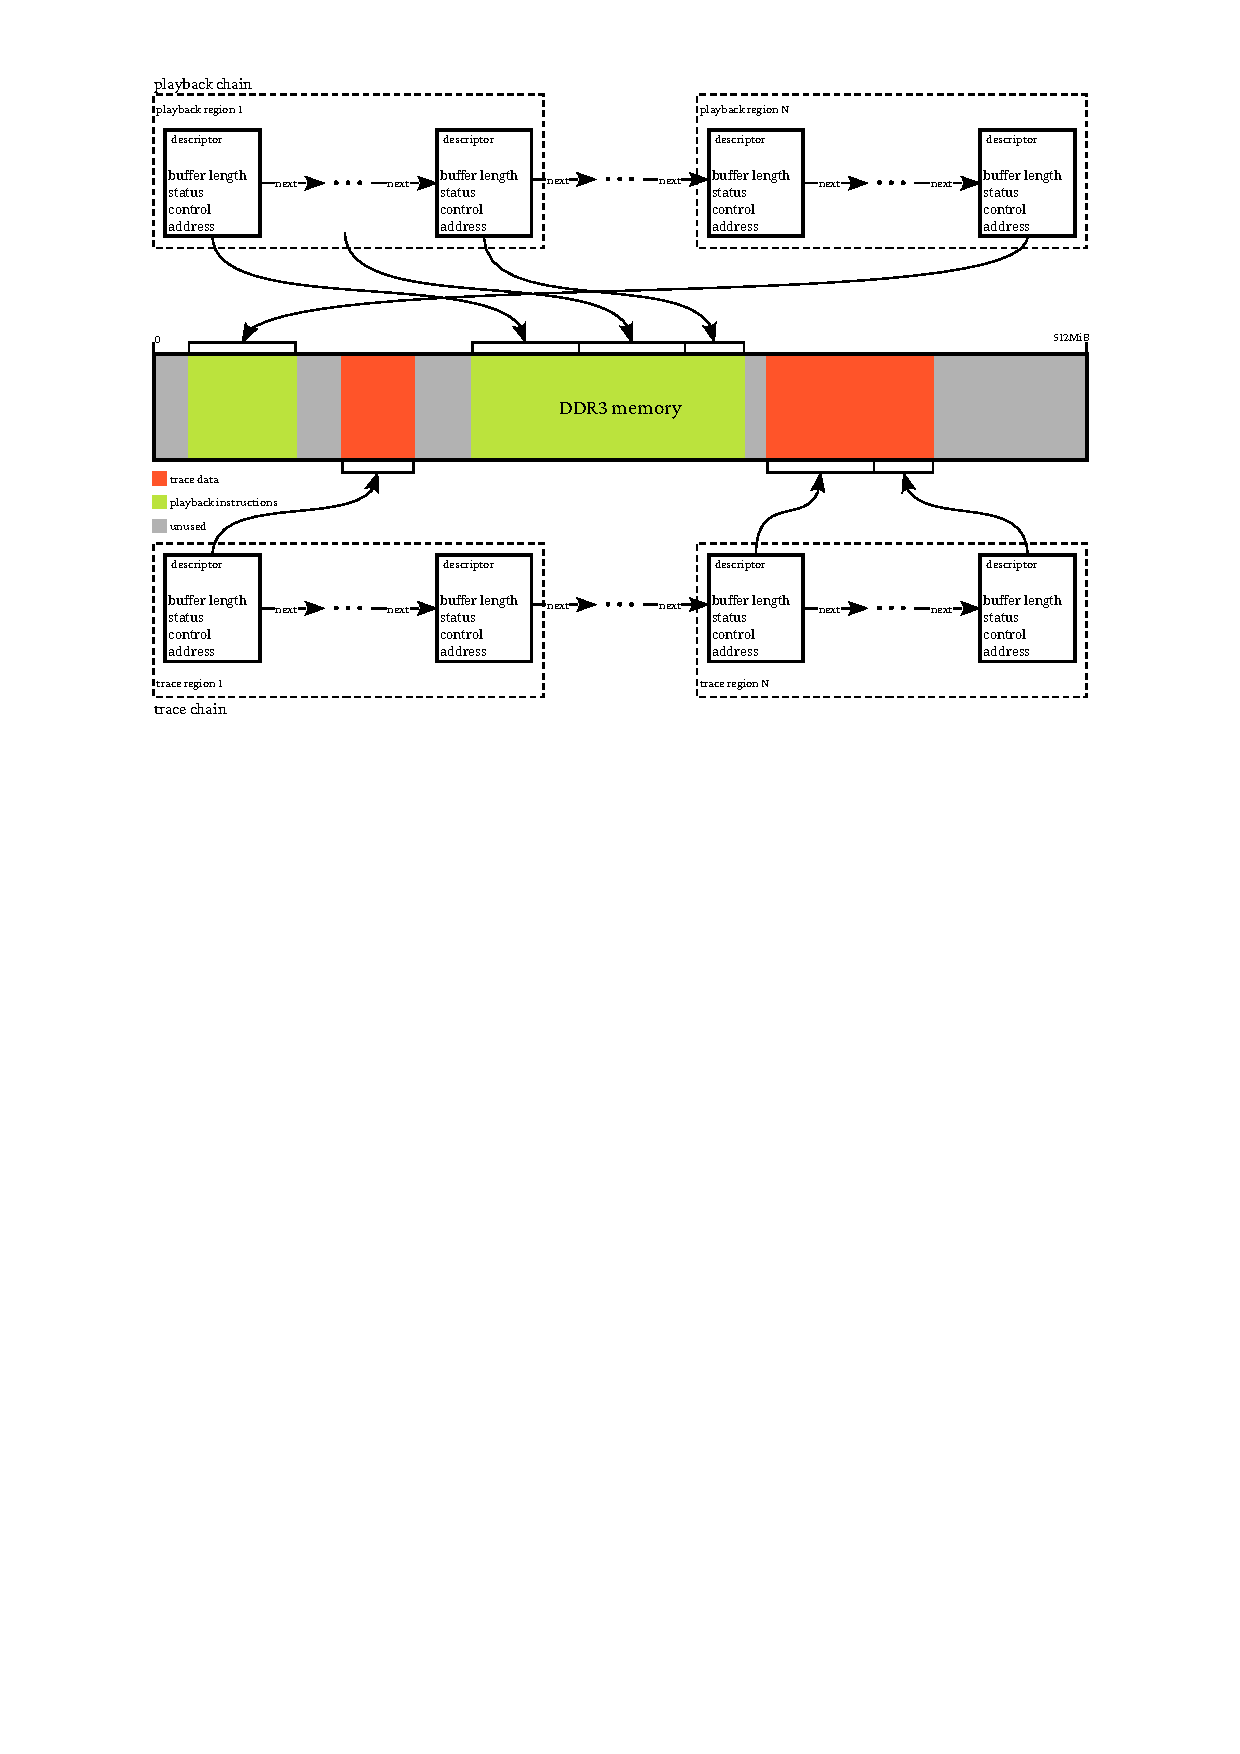
\includegraphics{diagrams/cropped/ayo_chain_detail}}
\caption{Schematic overview of an example for the playback and trace descriptor chains created for a set of playback and trace regions. In this example two playback regions were specified. The first playback region contains more than twice the maximum permissible buffer length for a single \descriptor{} and is therefore converted into a chain of three descriptors. The second playback region is small enough for one \descriptor{} to be sufficient. Note that the first playback region is stored after the second in the memory, but due to the order of the playback descriptors, the first playback region will be transmitted to the \pbexec{} before the second one. This example also has two trace regions, the first being small enough to be described by a single \descriptor{} and the second needing two \descriptor{}s. The order of the playback and trace regions in the \DDR{} memory is independent of the order they are actually used in.}\label{fig:ayo_chain_detail}
\end{figure}

The rate of experiments that can be performed in a \HWinTheLoop{} style operation, where each \PlaybackProgram{} depends on the trace data of the previous \PlaybackProgram{} is expected to be limited mainly by the round trip time between the host and the \FPGA{}. The old playback and trace buffer design requires just one round trip from the host to the \FPGA{}. It sends the \PlaybackProgram{} and then receives the trace data as it is generated.
To perform a single experiment with the new playback and trace buffer design five steps need to be performed
\begin{enumerate}
    \item\label{step:exec_first} The \PlaybackProgram{} is written to the \DDR{} memory
    \item A descriptor{} chain for the \PlaybackProgram{} and the memory region that captures the trace data is written to the \descriptor{} memory
    \item\label{step:exec_third} Operation of the \SToMM{} and \MMToS{} channels of the \AXIDMA{} is started by writing the proper \descriptor{} chain addresses to the \curdesc{} and \taildesc{} descriptors.
    \item The status field of the \descriptor{}(s) for the trace data is polled to determine when the \PlaybackProgram{} has finished execution as well as the size of the generated trace data.
    \item The trace data is read from the \DDR{} memory.
\end{enumerate}
The first two steps need to be completed before the third step is performed to guarantee both the playback and the descriptor data was written before it is read by the \AXIDMA{} unit.
A naive implementation would wait for the reception of the write response for the first two steps until it continues with the third step, but using the special \globalfence{} operation of the \FAXI{} block \ayo{} does not have to wait for response to the write operations in steps \autoref{step:exec_first} to \autoref{step:exec_third} and can instead ensure the write operations for the first two steps was completed before the \AXIDMA{} unit will be configured and in turn the data written in the first two stes will be read by the \AXIDMA{} by inserting a \globalfence{} operation before the write operations that configure the \AXIDMA{}. It is however unavoidable to wait for the response to the read operations that poll the status field of the trace \descriptor{}s, as the response data is used to determine when the readout of the trace data can be started as well as determining the size of the generated trace data. For an experiment with a single trace descriptor the lowest number of round trips that are necessary is therefore the number of times the status field has to be read until the \PlaybackProgram{} is completed plus one round trip for the readout of the trace data yielding a minimum of two round trips.
Accordingly, in the case of \HWinTheLoop{} style operation with small \PlaybackProgram{}s it is expected that the rate of experiments is at most half of the rate that can be achieved with the old playback and trace buffer design.
Future extensions of the playback and trace buffer design could reduce the number of roundtrips required again, by for example introducing a separate channel for the trace data, that bypasses the trace buffer and directly sends the trace data to the host.
\subsubsection{Allocator}
With the old FIFO based system, the \VFIFO{} module in the \FPGA{} is responsible for placing the playback data in the \DDR{} memory, reading it again from the address it was placed at, and vice versa for the trace data.
Changing the host interface to be memory mapped instead of FIFO based shifts the responsibility deciding the placement of the playback and trace data from the \FPGA{} to the host.
Furthermore, the playback data is no longer accessed in a strictly FIFO way, but instead can be built up from multiple blocks, with some blocks potentially being used by multiple experiments.
Management of the memory is abstracted by \ayo{} which simply presents the higher layers with the \code{alloc} and \code{free} functions that are used to reserve regions of memory and mark them as unused again.
In the \ayo{} layer tracking which regions of memory are already used for playback or trace data as well as allocating new regions or marking previously used regions as unused is done by an \allocator{}, which in turn provides the address for each of the memory regions. Its interface is described in \autoref{listing:allocator_interface}.

On creation, the allocator is given the size of the memory used for the playback and trace. Its \code{alloc} function finds an unused region in the memory that has at least a size of \code{size} bytes and returns the address of the first byte in this region.
When a memory region is no longer needed it can be marked as free again by calling the \code{free} function with the address of the first byte of the region.
Furthermore, the sum of the size of all unused regions can be queried using the \code{available_space} function.

% Memory allocators used by programming languages such as \c{} or \cpp{} also provide a function to resize a allocated region $R_{\text{old}}$. It provides the same operation as allocating a new region $R_{\text{new}}$ with the new size, copying the data from the old region to the new region and then freeing the old region, but can avoid copying the data if there is a free region of memory directly after the old region with sufficient size.
% This function is not provided by the allocator implemented here, as the allocator cannot directly access the memory and in turn cannot copy the data if necessary.

Layers using the \ayo{} layer provide the \ayo{} layer with a specific implementation of the allocator. A default implementation is provided by the \ayo{} layer. In the default implementation the allocator keeps a single list of free regions and allocas regions from this list using a best-fit strategy. When freeing a region creates consecutive free regions they are combined to form a larger free region. This implementation was chosen for its simplicity while being sufficient for all tests performed in this thesis.
\begin{listing}
\begin{minted}{c++}
template <typename T>
concept Allocator = requires(T allocator, size_t maximum_size, size_t size, size_t pointer)
{
	{ T(maximum_size) } -> std::same_as<T>;
	{ allocator.alloc(size) } -> std::same_as<size_t>;
	{ allocator.free(pointer) };
	{ allocator.available_space() } -> std::same_as<size_t>;
};
\end{minted}
\caption{Interface of the allocator. An allocator is give the size of the memory region it manages on creation. The \code{alloc} function is used to find a region of memory that is not yet marked as used by previous calls to \code{alloc} that fits atleast $\code{size}$ bytes. The offset of the first byte of this region from the start of the complete memory is returned. This offset will also be called the \code{pointer} to this region. Using the \code{free} function a region of memory is marked as unused again. It is called with the \code{pointer} to a memory region. Finally the \code{available_space} function returns the number of bytes that are not part of memory regions marked as used.}
\label{listing:allocator_interface}
\end{listing}

\subsection{Verification and comparison}
The correct operation of the new playback and trace buffer as well as the \ayo{} layer integrating it into the \BSSTwo{} software architecture is verified at different layers using unit and integration tests. Moreover, various performance aspects of the old and the new playback and trace buffer design are compared.

\subsubsection{Playback and trace buffer}
At the lowest level the correct operation of the playback and trace buffer that is part of the \FPGA{} design is verified on its own using simulation with the \xcelium{} simulator.
Writing simulation test benches for \FPGA{} cores can be done in a variety of ways, which can be broadly classified into two categories
\begin{itemize}
    \item Writing test benches in a \hdl{} for example using the \uvmframework{}\autocite{ref:uvm}.
    \item Writing test benches in a programming language and using a Co-simulation interface like \VPI{}\autocite{ref:vpi} or \DPI{}\autocite{ref:dpi} to interact with the simulated \FPGA{} core.
\end{itemize}
For verification of the standalone playback and trace buffer the \cocotb{} framework was used. This is a Co-simulation framework that uses the \VPI{} and \VHPI{}\autocite{ref:vhpi} interface to allow writing test benches using the \python{} programming language. Using \cocotb{} has multiple advantages, the \cocotbaxi{} module provides abstractions for using \AXI{}, like \AXI{} and \AXIStream{} Transmitter and Receiver implementations, as well as the \AXIRAM{} module, an \AXI{} Subordinate that implements a \RAM{}. Using these abstractions, the \HostARQ{} read and write, as well as the playback and trace streams are replaced with \AXIStream{} Transmitters and Receivers from the \cocotbaxi{} module and the \AXI{} \DRAM{} controller is replaced by the \AXIRAM{} module.
Furthermore, using \python{} makes it possible to use the rich ecosystem of \python{} modules to perform various tasks. In this test bench the \construct{}\autoref{ref:construct} module was used to perform serialization and deserialization of the bit fields that have to be created to interact with the \FAXI{} or the \AXIDMA{} module.

\subsubsection{flange-dram}
The communication layer of the \bssTwoOS{} presents higher level software with an unified interface for different communication backends (see \autoref{fig:bss_stack}). This allows all software using \hxcomm{} to transparently switch between interacting actual hardware and simulated hardware. In the simulated case, communication between the \hxcomm{} and the simulator simulating a combination of the \FPGA{} design and the \ASIC{} is facilitated using the \flange{} library.

\flange{} consists of two parts. The first part is a library that is loaded by the simulator. This library interacts with the simulator using the \DPI{} interface and exposes functions acting as stream Receiver and a stream Transmitter, as well as functions to schedule special actions in the simulation like stopping or resetting the simulation. The stream Transmitter and Receiver are used to replace the \HostARQ{} block and are connected to the input and output stream ports of the playback and trace buffer. An \RCF{}\autocite{ref:rcf} based network server exposes the special actions as well as reading or writing to the streams to the second part of \flange{}, which uses these to remotely control the simulation.

For the simulation there are two different models of the \AXI{} accessible \DRAM{} that can be selected. The first uses the same \MIG{} as used for synthesis and connects it to a \DDR{} simulation model provided by micron\autocite{ref:ddr3Model}. The second option replaces the \MIG{} and the \DDR{} model with an \AXIBRAMController{} connected to a behavioural model of a chain of Block-RAMs. While the first option offers a more accurate simulation it reduces the simulation performance. The second option allows for a faster simulation, but in addition to being less accurate also only models a size of \SIMMEMSIZE{} instead of the actual \DDRSIZE{} present on hardware.

To test \ayo{} correctly interacts with the \FAXI{} and \AXIDMA{} blocks it is useful to be able to test interaction with the \FAXI{} and the \AXIDMA{} block separately. This is only possible if the \DRAM{} that is access by both can be access by the test suite without using \FAXI{}. In a simulation environment there are several options for this:

\begin{itemize}
  \item Exposing an interface to the test suite to interact with the design hierarchy. This could for example use \VPI{} to allow enumeration, read and writing of all verilog signals. Using this interface the test suite could read or write to the signals corresponding to the memory of the \DRAM{} simulation model. This interface has several advantages. It does not need any modification of the simulated design and is general enough to be used with both the \AXIBRAMController{} based model and the \MIG{} based model. Furthermore, this interface could also be used for verification of other components that need access to signals in the design hierarchy. The main disadvantage is that this interface couples the test suite and the \FPGA{} design more tightly, because the test suite no longer only accesses the top level ports of the design, but can access any signal in the \FPGA{} design.
  \item Exposing an interface to the test suite that allows the test suite to act as an \AXI{} Manager and interact with the simulation. Using an \AXI{} interconnect the rest of the \FPGA{} design and this \AXI{} Manager could be connected to the \AXI{} \DRAM{} simultaneously. This option also does not need any modification to the \AXI{} \DRAM{} simulation model. In addition to that it could also be extended to be usable outside of simulation and in turn making the test suite usable with simulation and in hardware by using a synthesizable \AXI{} Manager that is accessible over a side band communication method like \JTAG{} in hardware.
  \item The choice of implementation of the \AXI{} \DRAM{} simulation model could be extended with a third option, that exposes the content of the memory to the test suite directly to \flange{}. This has the advantage of offering a fast simulation and the ability to simulate the whole \DDRSIZE{} of memory. However, it of course cannot be used together with one of the other options for the \AXI{} \DRAM{} simulation model, specifically the more accurate \MIG{} and \DDR{} simulation model based option, and therefore offers a less accurate simulation, effectively mocking out the RAM.
\end{itemize}
In this thesis the last option was chosen for its increased simulation performance and ability to simulate a memory with the same size as the actual memory present on the hardware. The \flangedram{} extension of \flange{} that exposes an \AXI{} Subordinate interface to the simulated \FPGA{} design and an interface to the test suite that allows for reading from and writing to the underlying memory was developed.
It is implemented using a \systemverilog{} and a \cpp{} part work together via \DPI{}. \autoref{dia:flange-dram-overview} shows an overview of its implementation. The \systemverilog{} part is realized in \code{dpi_axi_ram} module. This module creates a new memory using the \code{create_axi_ram} function of the \flangedram{} library exposed to the module via \DPI{} and receives a unique \code{id} identifying this memory. It collects transactions on the \AW{}, \AR{} \AXI{} channel and complete bursts on the \W{} \AXI{} channel. These transactions and bursts are transferred to the \cpp{} part using \DPI{}. Furthermore, it receives \B{} transactions and \R{} bursts from the \cpp{} part and writes these to the respective \AXI{} channels. Each instantiation of the \code{dpi_axi_ram} module creates a separate memory with a configurable size and address as well as data width.
The \cpp{} part manages the backing memory. The backing memory is allocated using \mmap{}, which, if memory overcommitment is enabled, allows simulation of very large memories, while only using physical memory for the pages that are actually written to. It receives \AW{} transactions and \W{} bursts, matches them together, writes the data to the backing memory and generates a corresponding \B{} response, as well as receives \AR{} transaction, reads the corresponding data from the backing memory and generates an \R{} burst. \autoref{tbl:flange-dram-featureset} summarizes the supported \AXI{} features. Finally, reads and writes to the backing memory are exposed to the test suite using the \RCF{} framework already used by \flange{}.
The correct operation of \flangedram{} itself was again verified with a test suite using the \AXI{} Manager provided by \cocotb{}

\begin{table}
  \begin{center}
\begin{tabular}{ll}
  \toprule
  feature & status \\
  \midrule
  data width & $8 · 2^{n}, n ∈ ℕ_{0}$ bits \\
  address width & $<= 64$ bits \\
  transaction ID & not supported \\
  AxLOCK & not supported \\
  AxCACHE & not supported \\
  AxPROT & not supported \\
  AxQOS & not supported \\
  AxREGION & not supported \\
  user signals & not supported \\
  narrow transfers & not supported \\
  \bottomrule
\end{tabular}
  \end{center}
\caption{Summary of the \AXI{} features supported by \flangedram}\label{tbl:flange-dram-featureset}
\end{table}

\begin{figure}[htbp]
\centerline{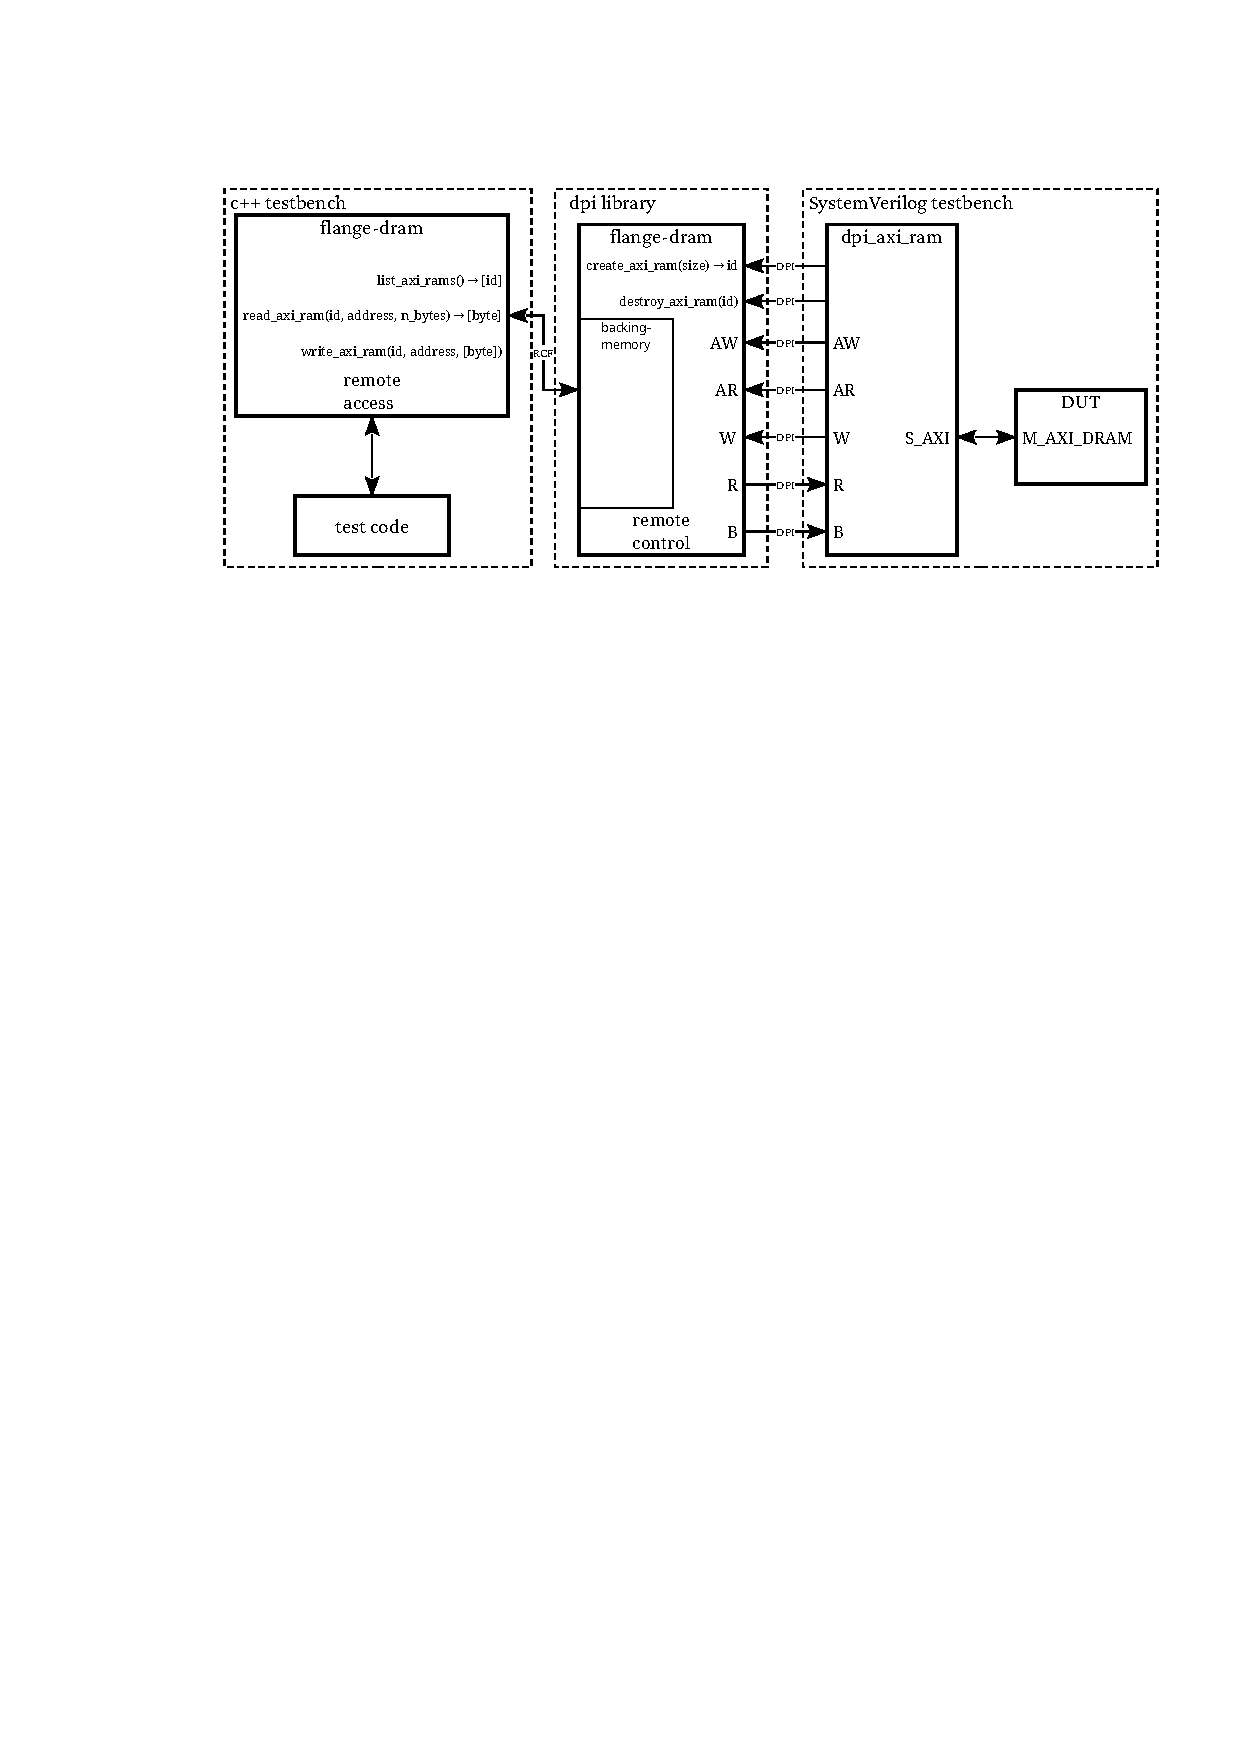
\includegraphics{diagrams/cropped/flange_dram}}
\caption{Schematic overview of \flangedram{} and its interaction with the \cpp{} test suite as well as the \systemverilog{} \DUT{}. \flangedram{} is split into two halves tha communicate via the \RCF{} remote procedure call framework. The first half is a \DPI{} library that exports several functions to be used by the \systemverilog{} code. \code{dpi_axi_ram} is a \systemverilog{} module that has an \AXI{} Subordinate interface and uses the functions exported by the \flangedram{} \DPI{} library to translate the \AXI{} read and write transactions to read and write operations on memory allocated by the \flangedram{} library. This module uses the \code{create_axi_ram} function to create a new memory and receives a \code{id} that identifies this memory. Transactions received on the \AW{}, \AR{} and \W{} \AXI{} channels are communicated to the \DPI{} library, using the \code{id} to identify the memory that they are targeting. Read and write response data is received using the \code{R} and \code{B} functions and converted to transfers on the \R{} and \B{} channels. Every instantiation of the \code{dpi_axi_ram} module creates a separate memory that can have different total sizes of the memory and different \AXI{} data widths.
The second half of \flangedram{} is a library used by the \cpp{} testbench to read and write the contents of the memories created by the \DPI{} library. Using the \code{list_axi_rams} function a list of the \code{id}s corresponding to the memories created by the \DPI{} library can be obtained and the \code{read_axi_ram} and \code{write_axi_ram} are use to read and write from a memory identified by the \code{id}.  }\label{dia:flange-dram-overview}
\end{figure}

\subsubsection{Bandwidth verification}\label{sec:pb_trace_verif}
The new playback and trace generator was designed to be able to sustain the maximum possible bandwidth of the trace and playback streams. However, without verification of this in hardware it is impossible to determine if it is actually able to achieve this bandwidth, due to the limited information on the performance of the \AXIDMA{} and the \XilinxMIG{} given.

For the \AXIDMA{} it is expected it can process the \descriptor{}s at a fixed rate $R$ that is slower than $1$ descriptor per clock cycle. This means that if a sufficiently low buffer length with each \descriptor{} is used the bandwidth of the playback and trace streams will not be limited by the \XilinxMIG{} but instead by this rate $R$.
The minimal buffer length $L$ for which the full playback and trace bandwidth could be reached is then
\[L = \frac{B_{\text{pb\_trace}}}{R}\]
Where $B_{\text{pb\_trace}}$ is the number of bytes that can be transmitted on the playback and trace streams per clock cycle, here $B_{\text{pb\_trace}} = \SI{8}{\byte}$.

To verify the actually achieved bandwidth the \pbexec{} was extended by a dummy data generator. This dummy data generator can be programmed using the \emitDummyInstr{} to emit the programmed number of words on the trace stream. The payload for this dummy data is  an \FPGA{} internal counter that increments with every clock cycle of the \pbexec{} called \systime{}. Dummy words are given the highest priority in the \traceArb{}.
The dummy data generation is mainly used to verify the bandwidth of the trace stream. To verify the bandwidth of the playback stream an instruction that can be processed by the \pbexec{} on every cycle is and has no unwanted side effect is chosen. In this case the \resetSleepInstr{} was used. It resets a counter internal to the \pbexec{} that is not used by the experiments performed here. Finally, every instruction and trace data word used in these experiments has a \UT{} encoding of exactly one \PhyWordSize{} word giving a one to one correspondence between the encoded and the unencoded playback instruction and trace data streams.

The first scenario that is investigated is the maximum bandwidth that can be achieved by the playback stream while minimal trace data is generated while varying buffer length $L$ of the \descriptor{}s used. The \descriptor{} memory has place for $\num{2048}$ \descriptor{}s. One \descriptor{} is needed for the trace data that will contain the value of the \systime{} counter when the first and the last playback instruction was executed, and an additional \descriptor{} is necessary to hold the \haltInstr{} used to mark the end of a \PlaybackProgram{}. This leaves $\num{2046}$ \descriptor{}s that are filled with playback instructions. The first and last playback instruction are \emitDummyInstr{} that each cause the dummy data generator to emit a single dummy word. A single clock cycle is require to execute them and the value of the dummy words is the value of the \systime{} counter when they were generated, which is used to determine value of \systime{} counter when the first and the last playback instruction was executed. All other playback instructions are filled with the \resetSleepInstr{}. The buffer length of each descriptor is varied by varying the number of words $N$ contained in the memory region used by each \descriptor{}. \autoref{fig:pb_benchmark_setup} shows a diagram of the \descriptor{} chains that are generated for this scenario.

As described in \autoref{sec:AXIDMA} the access pattern of a \DDR{} memory can have an influence on the read and write bandwidth that can be achieved. To investigate this effect three different placements of the playback instructions were used:

\begin{enumerate}
    \item With the \linear{} placement all playback instructions are located in the \DDR{} memory in the same order they are executed and therefore read from the memory.
    \item With the \random{} placement the location of each region of memory used for each \descriptor{} is randomized.
    \item With the \randomDense{} placement the location of each region of memory used for each \descriptor{} is randomized, but no gaps are allowed.
\end{enumerate}

\begin{figure}[htbp]
\centerline{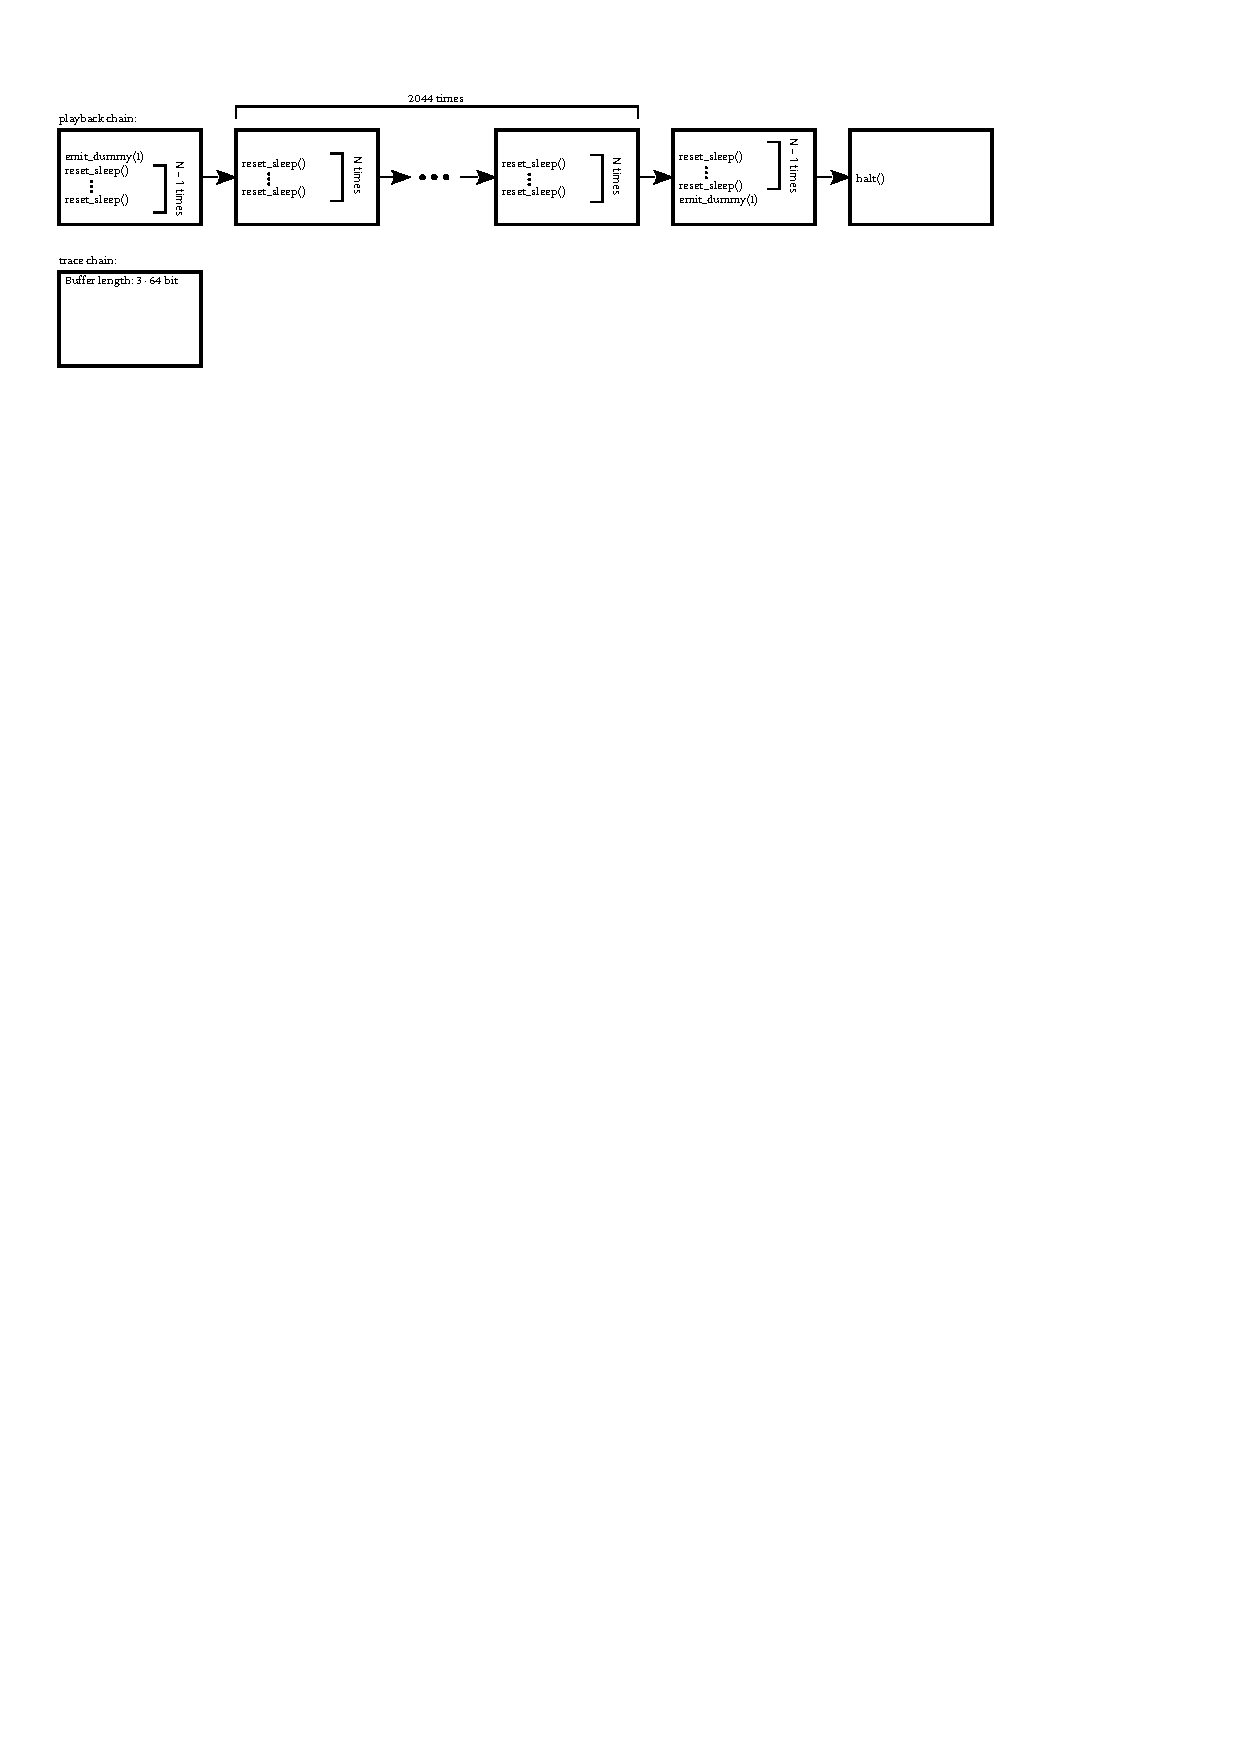
\includegraphics{diagrams/cropped/benchmark_pb}}
\caption{Schematic overview of the playback and trace buffer chains used to measure the playback bandwidth.}\label{fig:pb_benchmark_setup}
\end{figure}

The second scenario investigates the maximum bandwidth that can be achieved by the trace stream while minimal words are transmitted on the playback stream. A single \descriptor{} is used for the playback stream, that first configures a long timeout to avoid interruption of the generation of the dummy trace data by a timeout notification. It configures the dummy data generator to generate dummy trace data and after waiting for the dummy data generator to be idle terminates the \PlaybackProgram{} using the \haltInstr{}. The looped back \haltInstr{} is received by its own trace \descriptor{}. The other $\num{2046}$ trace descriptors are configured in one single \descriptor{} chain. The number of words $N$ that is received by each \descriptor{} is varied. Finally, for the placement of the trace memory region used by each of the \descriptor{} the same three placement strategies as for the first scenario are used. In this case the number of clock cycles that were needed to receive the whole trace data can be determined by comparing the \systime{} value of the first and the last dummy word that is written to the trace memory. \autoref{fig:trace_benchmark_setup} shows an overview of the \descriptor{} chains used in this scenario.

\begin{figure}[htbp]
\centerline{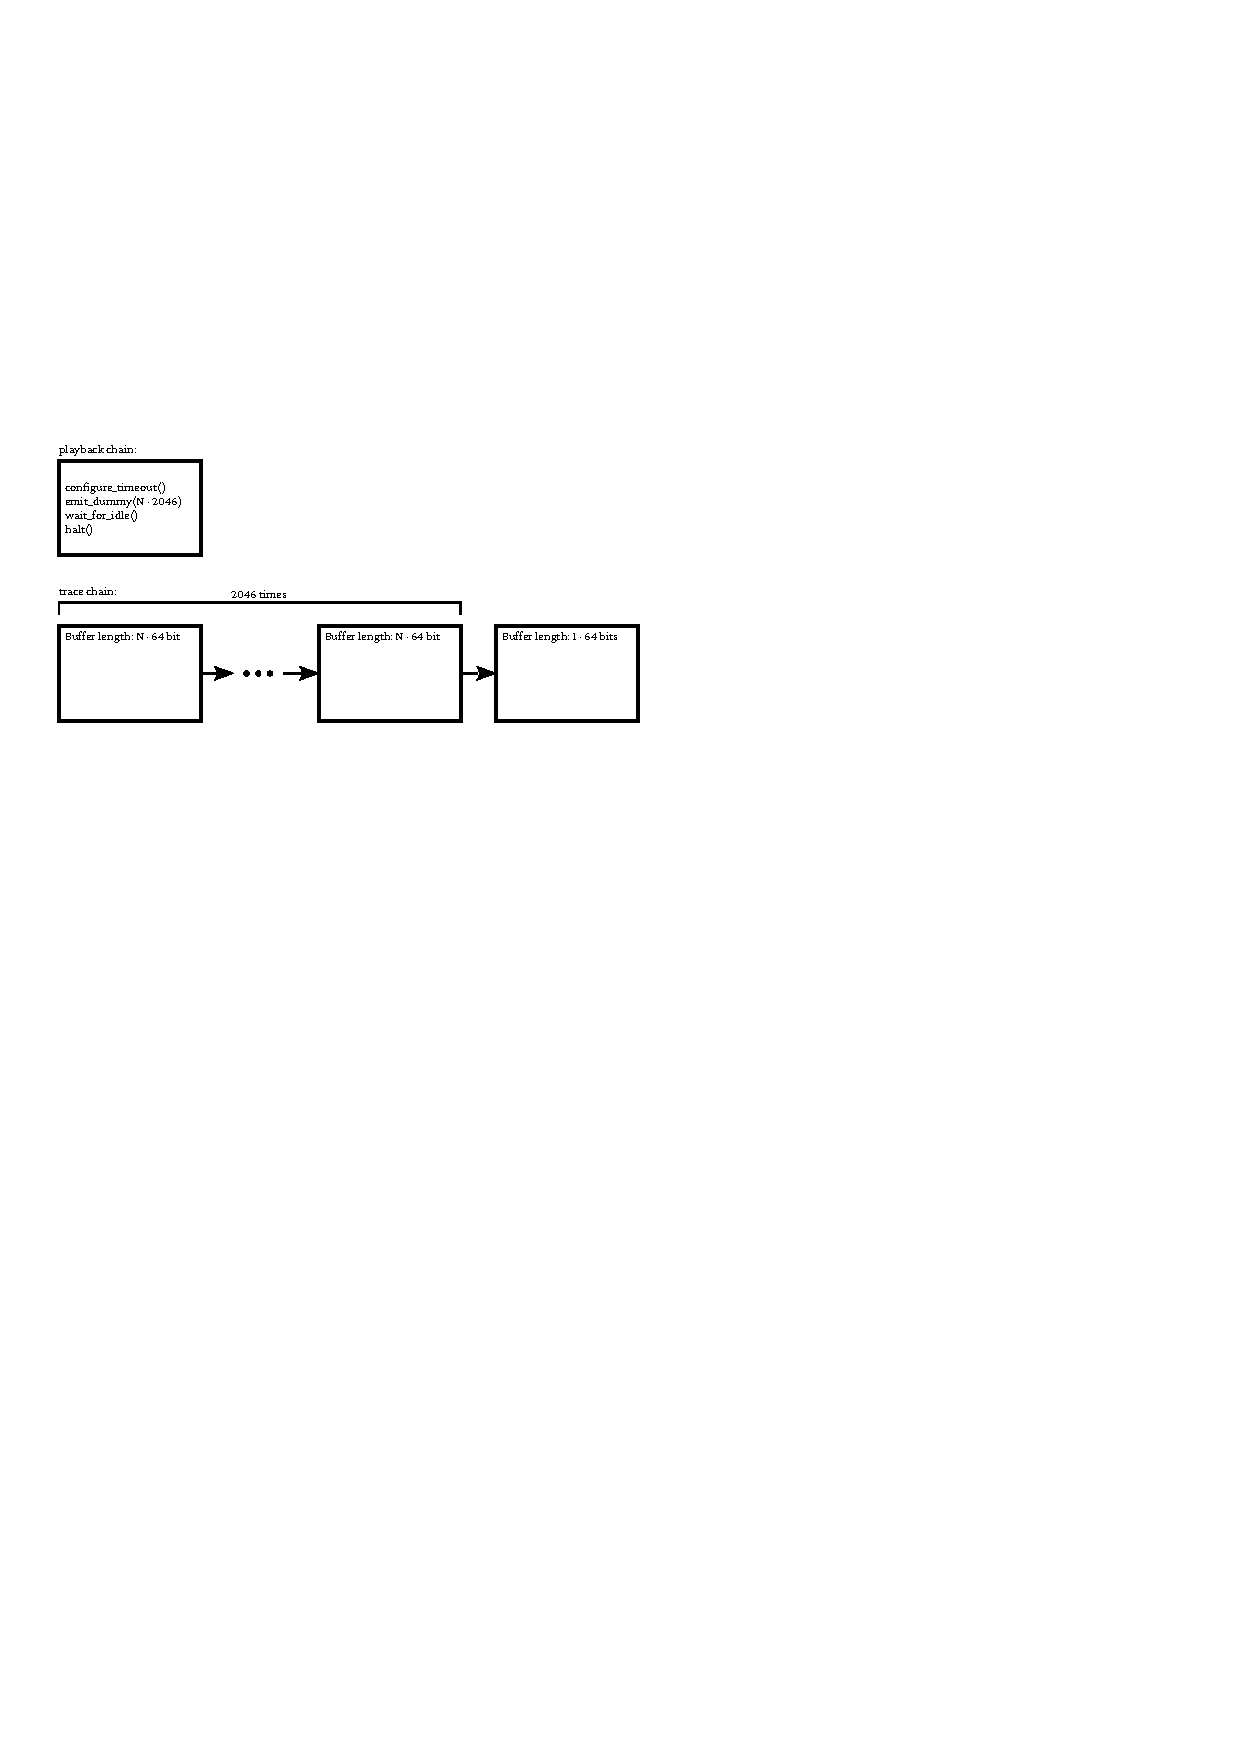
\includegraphics{diagrams/cropped/benchmark_trace}}
\caption{Schematic overview of the playback and trace buffer chains used to measure the trace bandwidth}\label{fig:trace_benchmark_setup}
\end{figure}

At last the third scenario measures the maximum bandwidth achieved on the playback and trace streams when both are used at the same time. Using the dummy data generator the \pbexec{} is configured to generate the same number of trace words as it will receive playback instructions. One playback \descriptor{} is used in the beginning to configure the timeout already mention in the second scenario. Furthermore, an additional \descriptor{} is used for the playback chain that contains the \haltInstr{} used to indicate the end of a \PlaybackProgram{}, which is looped back to a third \descriptor{} used in the trace chain. The remaining $\num{2045}$ are split evenly between the playback and the trace chain. One \descriptor{} stays unused. The first instruction in the playback stream after the timeout configuration configures the dummy data generator to emit the number of dummy words necessary to fill the trace \descriptor{} chain, while the last instruction before the \haltInstr{} causes \systime{} counter to be read from  an \FPGA{} internal bus. This will cause the value of the \systime{} counter one clock cycle after it was executed to be placed into a \FIFO{} internal to the \pbexec{} where it will remain until it can be written to the trace stream. As the dummy data generator has the highest priority this can only happen after all dummy data was generated and therefore does not influence the trace stream. \autoref{fig:pb_trace_benchmar_setup} gives an overview of the playback and trace chains that are generated for this case.

In this case again the number of words $N$ used in each \descriptor{} and the placement of the playback instructions and the trace data varied.
Here five different configurations for the placement were investigated:
\begin{enumerate}
  \item \linear{} placement, that places all playback instructions is the same order as they are executed, and also places the trace data for each \descriptor{} consecutively.
  \item \random{} placement that randomizes the location of each region of playback instructions and trace data
  \item \randomDense{} placement that randomizes the location of each region of playback instructions and trace data while not leaving any gaps
  \item \interleaved{} placement that places the playback instructions and the trace data into alternating regions leaving gaps between each of them
  \item \interleavedDense{} placement that places the playback instructions and the trace data into alternating consecutive regions
\end{enumerate}

\begin{figure}[htbp]
\centerline{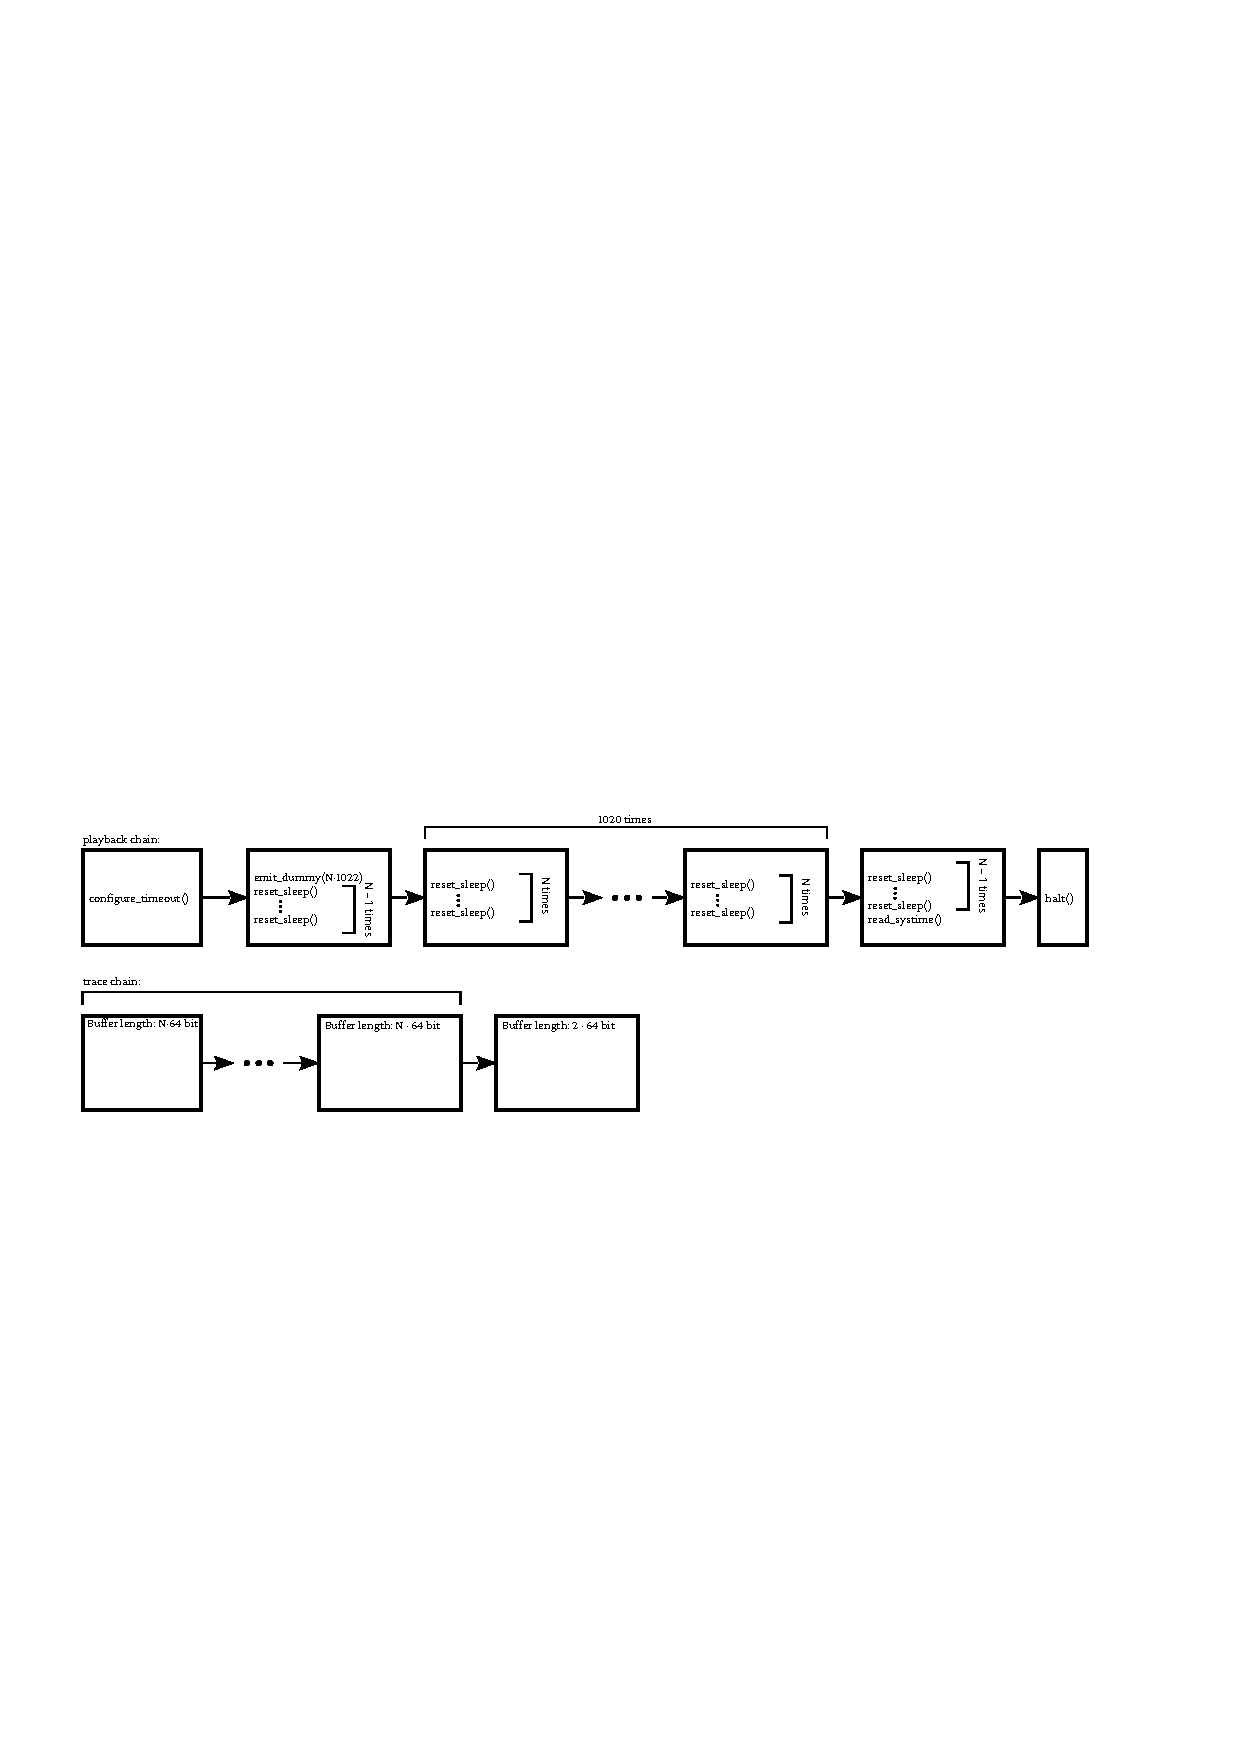
\includegraphics{diagrams/cropped/benchmark_pb_trace}}
\caption{Schematic overview of the playback and trace buffer chains used to measure simultaneous playback and trace bandwidth}\label{fig:pb_trace_benchmar_setup}
\end{figure}
